\documentclass[tikz,border=6pt]{standalone}
\usepackage[scaled]{helvet}
\renewcommand\familydefault{\sfdefault}
% Shared TikZ style for every project diagram (README figures and the manuscript).
\usepackage{amsmath,amssymb}
\usetikzlibrary{arrows.meta,positioning,fit,backgrounds,calc,shapes.geometric,decorations.pathreplacing}
\definecolor{cam}{HTML}{2563EB}     % endoscope / camera action
\definecolor{armA}{HTML}{EA580C}    % instrument arm USM1
\definecolor{armB}{HTML}{16A34A}    % instrument arm USM3
\definecolor{armC}{HTML}{9333EA}    % instrument arm USM4
\definecolor{ink}{HTML}{1F2937}
\definecolor{muted}{HTML}{6B7280}
\definecolor{panel}{HTML}{F3F4F6}
\definecolor{model}{HTML}{0F766E}
\tikzset{
  >={Stealth[length=2.2mm]},
  every node/.style={font=\sffamily\small, text=ink},
  box/.style={draw=ink!60, rounded corners=2pt, fill=white, inner sep=4pt, align=center, line width=0.5pt},
  data/.style={box, fill=panel},
  proc/.style={box, fill=model!8, draw=model!70},
  learn/.style={box, fill=model!20, draw=model, line width=0.8pt},
  sig/.style={box, font=\sffamily\scriptsize},
  group/.style={draw=muted!70, dashed, rounded corners=4pt, inner sep=6pt},
  flow/.style={->, line width=0.7pt, draw=ink!70},
  note/.style={font=\sffamily\scriptsize, text=muted, align=center},
  token/.style={draw, rounded corners=1pt, minimum width=5mm, minimum height=4mm, inner sep=1pt,
                font=\sffamily\scriptsize\bfseries},
}

\begin{document}
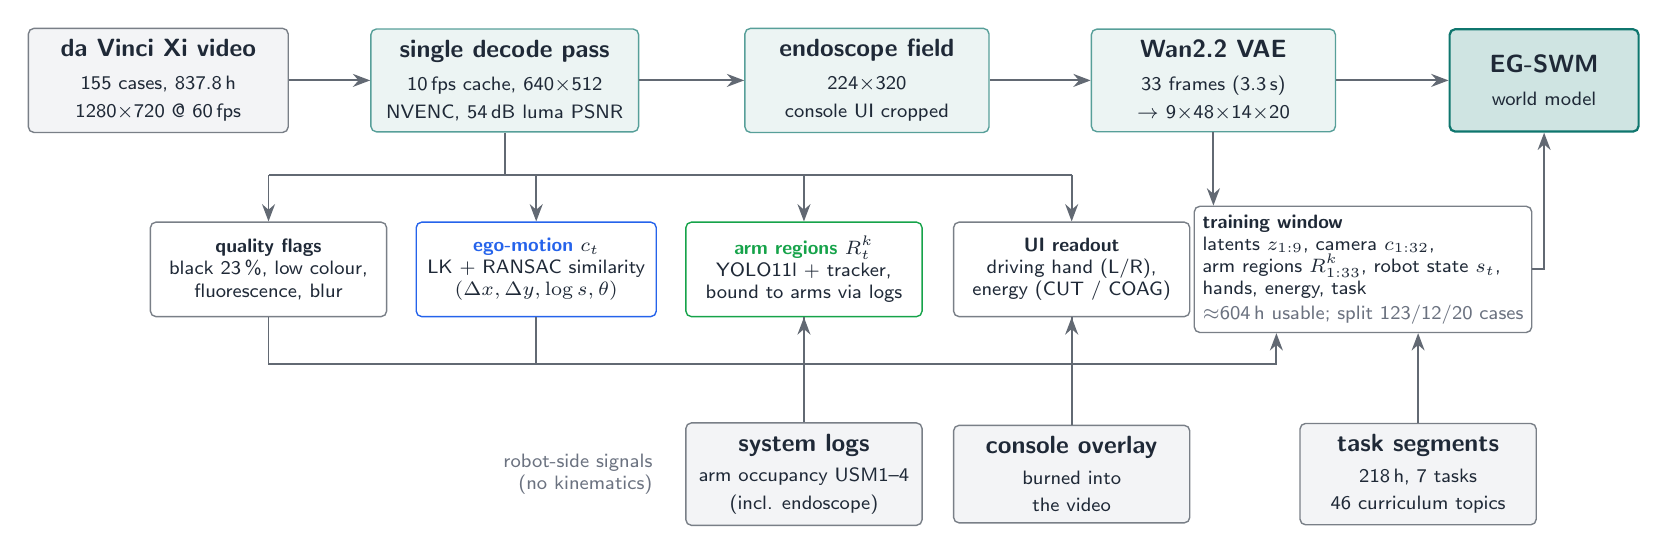
\begin{tikzpicture}[x=1mm, y=1mm]

% ---------------- row A: video path ----------------
\node[data, minimum width=33mm, minimum height=13mm] (video) at (0, 0) {\textbf{da Vinci Xi video}\\[1pt]
  {\scriptsize 155 cases, 837.8\,h}\\[-1pt]{\scriptsize 1280$\times$720 @ 60\,fps}};
\node[proc, minimum width=34mm, minimum height=13mm] (cache) at (44, 0) {\textbf{single decode pass}\\[1pt]
  {\scriptsize 10\,fps cache, 640$\times$512}\\[-1pt]{\scriptsize NVENC, 54\,dB luma PSNR}};
\node[proc, minimum width=31mm, minimum height=13mm] (field) at (90, 0) {\textbf{endoscope field}\\[1pt]
  {\scriptsize 224$\times$320}\\[-1pt]{\scriptsize console UI cropped}};
\node[proc, minimum width=31mm, minimum height=13mm] (vae) at (134, 0) {\textbf{Wan2.2 VAE}\\[1pt]
  {\scriptsize 33 frames (3.3\,s)}\\[-1pt]{\scriptsize $\to$ 9$\times$48$\times$14$\times$20}};
\node[learn, minimum width=24mm, minimum height=13mm] (wm) at (176, 0) {\textbf{EG-SWM}\\[1pt]{\scriptsize world model}};
\draw[flow] (video) -- (cache); \draw[flow] (cache) -- (field); \draw[flow] (field) -- (vae); \draw[flow] (vae) -- (wm);

% ---------------- row B: per-frame signals ----------------
\node[sig, minimum width=30mm, minimum height=12mm] (qual) at (14, -24) {\textbf{quality flags}\\ black 23\,\%, low colour,\\ fluorescence, blur};
\node[sig, minimum width=30mm, minimum height=12mm, draw=cam] (ego) at (48, -24) {\textbf{\textcolor{cam}{ego-motion} $c_t$}\\ LK + RANSAC similarity\\ $(\Delta x,\Delta y,\log s,\theta)$};
\node[sig, minimum width=30mm, minimum height=12mm, draw=armB] (det) at (82, -24) {\textbf{\textcolor{armB}{arm regions} $R^k_t$}\\ YOLO11l + tracker,\\ bound to arms via logs};
\node[sig, minimum width=30mm, minimum height=12mm] (ui) at (116, -24) {\textbf{UI readout}\\ driving hand (L/R),\\ energy (CUT / COAG)};
\draw[ink!70, line width=0.7pt] (cache.south) -- (44, -12) -- (14, -12);
\draw[ink!70, line width=0.7pt] (44, -12) -- (116, -12);
\foreach \n/\x in {qual/14, ego/48, det/82, ui/116} \draw[flow] (\x, -12) -- (\n.north);

% ---------------- training window ----------------
\node[box, minimum width=36mm, align=left, font=\sffamily\scriptsize, inner sep=3pt] (win) at (153, -24) {%
  \textbf{training window}\\
  latents $z_{1:9}$, camera $c_{1:32}$,\\
  arm regions $R^k_{1:33}$, robot state $s_t$,\\
  hands, energy, task\\[1pt] {\color{muted}$\approx$604\,h usable; split 123/12/20 cases}};
\draw[flow] (vae.south) -- (vae.south |- win.north);
\draw[ink!70, line width=0.7pt] (qual.south) -- (14, -36) -- (116, -36);
\foreach \x in {48, 82, 116} \draw[ink!70, line width=0.7pt] (\x, -30) -- (\x, -36);
\draw[flow] (116, -36) -- (142, -36) -- (142, -24 |- win.south);
\draw[flow] (win.east) -| (wm.south);


% ---------------- row C: robot-side sources ----------------
\node[data, minimum width=30mm, minimum height=11mm] (logs) at (82, -50) {\textbf{system logs}\\{\scriptsize arm occupancy USM1--4}\\[-1pt]{\scriptsize (incl. endoscope)}};
\node[data, minimum width=30mm, minimum height=11mm] (overlay) at (116, -50) {\textbf{console overlay}\\{\scriptsize burned into}\\[-1pt]{\scriptsize the video}};
\node[data, minimum width=30mm, minimum height=11mm] (tasks) at (160, -50) {\textbf{task segments}\\{\scriptsize 218\,h, 7 tasks}\\[-1pt]{\scriptsize 46 curriculum topics}};
\draw[flow] (logs.north) -- (det.south);
\draw[flow] (overlay.north) -- (ui.south);
\draw[flow] (tasks.north) -- (win.south -| tasks.north);
\node[note, anchor=east, align=right] at (64, -50) {robot-side signals\\ (no kinematics)};
\end{tikzpicture}
\end{document}
